\chapter{Spatially structured networks\label{ch:spatial}}

\graphicspath{{figs/spatial/}}


We will now describe the procedure for testing the probabilistic connection algorithms for spatially structured networks. We briefly discussed spatially structured networks in the introduction, and an example was show in Figure \ref{fig:spatial_example_intro}. In NEST, these connection patterns can be created between two- or three-dimensional layers using the function \inline{ConnectLayers} from the \inline{Topology} module \shortcite{plesser2012topo}.



\section{Two-dimensional space\label{sec:2D}}

Concepts and derivations in this section are based on \shortciteN{kriener2012testconn}. Let one node be centered on a quadratic $L \times L\label{eq:L}$ layer. It can connect to $N\label{eq:N}$ other nodes, uniformly distributed on the layer, as long as they are inside the mask. The mask has the same size as the layer, and for now, the same position. The probability of making a connection is given by a distance-dependent connection probability (kernel). Let $(x_i)_m$ be the $m$th component of the coordinate vector for node $i$. Let 
\begin{equation}\label{eq:Dij}
D_{ij} = \sqrt{\sum_{m=1}^k \left(\Delta x_{ij}\right)_m^2},
\end{equation}
where $k = 2$ is the number of dimensions, be the distance between nodes $i$ and $j$. With periodic boundary conditions, 
\begin{equation}
\left(\Delta x_{ij}\right)_m = 
\begin{cases}
|(x_i)_m - (x_j)_m| & \text{for } |(x_i)_m - (x_j)_m| \le L/2 \\
L - |(x_i)_m - (x_j)_m| & \text{for } |(x_i)_m - (x_j)_m| > L/2 \\
\end{cases}
\end{equation}

We wish to compare the observed distribution of distances between connected nodes with the expected distribution. The expected distribution depends on both on the number of potential targets at a given distance, and the probability of connecting to nodes at that distance (given by the kernel). We start by deriving an expression for the number of potential targets at a given distance. 

Let $\rho_0 = N/L^2\label{eq:rho0}$ be the average node density on the layer. Now consider a ring like the one in Figure \ref{fig:radial_distribution}, with radius $D$ and thickness $\mathrm{d}D$. 
\begin{figure}[t]
  \centering
  \includegraphics[width=0.65\textwidth]{radial_distribution.pdf}
  \caption[Illustration of the derivation of the expression for the radial distribution function]{A ring of radius $D$ and thickness $\mathrm{d}D$ is placed on a layer with a node density $\rho_0 = N/L^2$. The expected number of nodes inside the ring is then $\mathrm{d}N = \rho_0 \pi \left[ (D+\mathrm{d}D)^2-D^2\right]$.}
  \label{fig:radial_distribution}
\end{figure}
The expected number of nodes in the ring will be
\begin{gather}
\mathrm{d}N = \rho_0 \pi \left[ (D+\mathrm{d}D)^2-D^2\right]
\intertext{and the density of nodes in the ring is given by $\mathrm{d}N/\mathrm{d}D$. We now define the radial distribution function (RDF) as the limit of the node density for an infinitesimally thin ring}
\rho(D) = \lim_{\mathrm{d}D \to 0}\frac{\mathrm{d}N}{\mathrm{d}D}=2\pi\rho_0 D\;.\label{eq:radial}
\end{gather}
Thus, for distances $D \in [0, L/2]$ from the center node, the RDF is proportional to the circumference of a circle with radius $D$. For $D \in (L/2, L/\sqrt{2}]$, the mask comes into play, as part of the circle of radius $D$ is outside the mask.
\begin{figure}[h]
\centering
\begin{subfigure}[b]{0.49\textwidth}
	  \begin{flushleft}
	  \large A
		\end{flushleft}
    \centering
    \includegraphics[width=\textwidth]{mask.pdf}
    \phantomcaption\label{subfig:mask_radius}
\end{subfigure}
\begin{subfigure}[b]{0.49\textwidth}
	  \begin{flushleft}
	  \large B
		\end{flushleft}
    \centering
    \includegraphics[width=\textwidth]{mask_angles.pdf}
    \phantomcaption\label{subfig:mask_angles}
\end{subfigure}
\caption[The effect of the mask on the radial distribution function]{\subref{subfig:mask_radius}: Illustration of the effect of the mask on the radial distribution function (RDF). At distance $D_1$, the RDF is $\rho_0 2\pi D$. At distances $D \ge D_2$, the mask comes into play. At distance $D_3$, for example, part of the circle is outside the mask, and the number of nodes eligible for connecting to thus reduced. \subref{subfig:mask_angles}: The fraction of a circle with radius D which is inside the mask is $2\beta/\pi$. Adapted from \shortciteN{kriener2012testconn}.}
\label{fig:masks}
\end{figure} 
This is illustrated in Figure \ref{subfig:mask_radius}. As seen in Figure \ref{subfig:mask_angles}, only a fraction $2\beta/\pi$ lies inside the mask, where
\begin{equation}\label{eq:angle_beta}
\beta = \frac{\pi}{2} - 2 \alpha = \frac{\pi}{2} - 2 \, \text{arccos}\left( \frac{L}{2D} \right).
\end{equation}
Substituting for $\beta$ from \ref{eq:angle_beta} the fraction becomes
\begin{equation}
\frac{2\beta}{\pi} = \frac{\pi - 4 \, \text{arccos}\left( \frac{L}{2D} \right)}{\pi} .
\end{equation}
The RDF can therefore be summarized as
\begin{equation}
\rho(D) = 
\begin{cases}
   \rho_0 2 \pi D   &   \text{for } 0 \le D \le \frac{L}{2} \\ 
   \rho_0 2 D \left( \pi - 4 \, \text{arccos}\left( \frac{L}{2D} \right)\right)   &   \text{for } \frac{L}{2} < D \le \frac{L}{\sqrt{2}} \\
   0 & \text{otherwise}.
\end{cases}
\end{equation}

Let $\mathcal{P}(D)\label{eq:kernel}$ be a distance-dependent connection probability function (kernel). The probability density function (PDF) $f(D)$ of distances from the centered node and connected nodes is the normalized product of the RDF and the kernel, i.e., 
\begin{equation}\label{eq:f}
f(D) = \frac{\rho(D) \mathcal{P}(D)}   {\int_0^{L/\sqrt{2}}{ \rho(R) \mathcal{P}(R) \, \mathrm{d}R}},
\end{equation}
where the denominator is a normalizing constant\footnote{$R$ is used instead of $D$ in integrals as $D$ sometimes plays the role of the upper integration limit, for instance in Equation \ref{eq:F}.}.
The cumulative distribution function (CDF) $F(D)\label{eq:F}$ can be obtained by integrating $f(D)$, i.e.,
\begin{equation}\label{eq:F}
F(D) = \frac{\int_0^D \rho(R) \mathcal{P}(R) \, \mathrm{d}R}   {\int_0^{L/\sqrt{2}} \rho(R) \mathcal{P}(R) \, \mathrm{d}R}.
\end{equation}

As an example, let $L = 1$ and the kernel be a linear function of $D$, $\mathcal{P}(D) = (c - aD) H(c/a-D)$, where $H\label{eq:Heaviside}$ is the Heaviside step function. For simplicity we assume that $c/a < L/2$ so that there are no boundary effects. The PDF then becomes
\begin{equation}
f(D) = \frac{\rho_0 2\pi D (c-aD)}{\int_0^{c/a} \rho_0 2\pi R (c-aR) \, \mathrm{d}R}
= \frac{6a^2D(c-aD)}{c^3},
\end{equation}
and the CDF becomes 
\begin{equation}
F(D) = \frac{6a^2}{c^3} \int_0^D R(c-aR) \, \mathrm{d}R = \frac{a^2 D^2 (3c-2aD)}{c^3}.
\end{equation}
Using numerical integration, CDFs can be similarly found for other kernels. In Figure \ref{fig:2Dex}, an exemplary PDF and the corresponding CDF are shown, as well as the connectivity pattern of the network. A Gaussian kernel is used. 

\begin{figure}[ht]
\centering
\begin{subfigure}[b]{0.49\textwidth}
	  \begin{flushleft}
	  \large A
		\end{flushleft}
    \centering
    \includegraphics[width=\textwidth]{Gaussian1_PDF.pdf}
    \phantomcaption\label{subfig:gaussian_PDF}
\end{subfigure}
\begin{subfigure}[b]{0.49\textwidth}
	  \begin{flushleft}
	  \large B
		\end{flushleft}
    \centering
    \includegraphics[width=\textwidth]{Gaussian1_CDF.pdf}
    \phantomcaption\label{subfig:gaussian_CDF}
\end{subfigure}
\begin{subfigure}[b]{0.49\textwidth}
	  \begin{flushleft}
	  \large C
		\end{flushleft}
    \centering
    \includegraphics[width=\textwidth]{Gaussian1_network.png}
    \phantomcaption\label{subfig:gaussian_network}
\end{subfigure}
\caption[Exemplary PDF, CDF and connectivity pattern for a network in 2D space, using a Gaussian kernel]{Exemplary PDF (\subref{subfig:gaussian_PDF}), CDF (\subref{subfig:gaussian_CDF}) and connectivity pattern (\subref{subfig:gaussian_network}). A Gaussian kernel is used, and the layer and mask size is $L^2 = 1$. The sharp kink at $D = 0.5$ in the PDF is due to the mask. A kink exists in the CDF as well, marked by the arrow.}
\label{fig:2Dex}
\end{figure}

Using the two-sided KS test, the observed EDFs can now be compared with these theoretical CDFs, with the null hypothesis $H_0$ that distances are drawn from the theoretical PDFs. The KS test is the natural choice here because we are looking at the distribution of a continuous parameter, the distance.

As will be discussed in Section \ref{subsec:2D_res}, a few types of errors will not be detected by the KS test of the distribution of source-target distances. A second test is therefore implemented. It simply compares the total number of connections $C\label{C_spatial}$ with the expected number of connections $C_0\label{C_spatial0}$. $C$ will be the sum of $N$ independent Bernoulli random variables with different success probabilities $p$ given by the kernel. Its distribution is the Poisson binomial distribution, a generalization of the binomial distribution that does not require all success probabilities to be the same \shortcite{wang1993number}. For large $N$ it approximates the normal distribution $\mathcal{N}(\mu, \sigma^2)$, with $\mu = \sum_{i=1}^N{p_i}$ and $\sigma^2 = \sum_{i=1}^N{p_i(1-p_i)}$. 
The $Z$-test can thus be used as described in Section \ref{sec:z}. Using the test statistic
\begin{equation}
Z = \frac{C - C_0}{\sigma} = \frac{C - \sum_{i=1}^N{p_i}}{\sqrt{\sum_{i=1}^N{p_i(1-p_i)}}},
\end{equation}
the two-sided $p$-value $2\Prob{Z \ge \lvert z \rvert}$ can be calculated. 




\subsection{Implementation\label{subsec:2Dimp}}

An implementation of the test procedure described above is found in Appendix \ref{app:2D}. The main block at the bottom demonstrates the usage. The class \inline{ConnectLayers2D_tester} is first instantiated with the required arguments \inline{L} (side length of the square layer), \inline{N} (number of nodes), and \inline{kernel_name} (name of the kernel to use, ``constant'', ``linear'', ``exponential'', or ``gaussian''). An optional argument, \inline{kernel_params}, can be used to specify the parameters of the chosen kernel. Without this argument, sensible default values are used. The master seed value can be set using the optional argument \inline{msd}. The value of \inline{msd} is used to seed the PRNG used to draw the uniform, random positions for the nodes. NEST's global PRNG and each of the per-process PRNGs are seeded with the values (\inline{msd} $+$ $1$, \inline{msd} $+$ $2$, ..., \inline{msd} $+$ $n_\text{vp}+1$), where $n_\text{vp}$ is the number of virtual processes (VPs). Thus, for independent results, \inline{msd} should differ by at least $2+n_\text{vp}$ between each instantiation of the class. The position of the source node is (0, 0) by default, but it can be changed with the optional \inline{source_pos} argument. The mask is always centered around the source node, regardless of its position. 

After the test object is created, the KS test can be run using the \inline{ks_test} method. The KS test statistic and $p$-value is returned. The PDF is calculated on-the-fly as the product of the relevant kernel and the RDF. The CDF is then found by numerical integration, using the \inline{quad} function from the \inline{scipy.integrate} module. For finite integration limits the function uses the Clenshaw-Curtis method of numerical integration. 

The method \inline{z_test} implements the $Z$-test of the total connection count described earlier. The standard score and the two-sided $p$-value is returned.



\subsection{Results\label{subsec:2D_res}}

\graphicspath{{figs/spatial/2D_results/}}

The test script in Appendix \ref{app:2D} will now be used to test the connection algorithms for connecting 2D layers of spatially structured networks in NEST. 

With $L = 1$, $N =$ 1,000,000, and \inline{msd} $= 0$, and with the constant kernel selected, the distribution of distances to connected nodes is as shown in Figure \ref{fig:res_constant}. 
\begin{figure}[b]
\centering
\begin{subfigure}[b]{0.49\textwidth}
	  \begin{flushleft}
	  \large A
		\end{flushleft}
    \centering
    \includegraphics[width=\textwidth]{2D_constant_PDF.pdf}
    \phantomcaption\label{subfig:res_constant_PDF}
\end{subfigure}
\begin{subfigure}[b]{0.49\textwidth}
	  \begin{flushleft}
	  \large B
		\end{flushleft}
    \centering
    \includegraphics[width=\textwidth]{2D_constant_CDF.pdf}
    \phantomcaption\label{subfig:res_constant_CDF}
\end{subfigure}
\caption[Theoretical and empirical PDF and CDF of source-target distances using a constant kernel]{PDF (\subref{subfig:res_constant_PDF}) and CDF (\subref{subfig:res_constant_CDF}) of source-target distances, with layer size $L^2=1$, using a constant kernel. The grey lines show the theoretical predictions, and the red lines show the empirical observations. The empirical PDF is plotted with 100 bins.}
\label{fig:res_constant}
\end{figure}
There seems to be close agreement between the expected and observed distributions. According to the KS test, there is no evidence to reject the null hypothesis that the distances are drawn from the theoretical PDF ($p = 0.321$). Similar results are found for the linear ($p = 0.837$), exponential ($p = 0.630$) and Gaussian ($p = 0.852$) kernels. 

By positioning the source node away from the center, while leaving the mask centered around the node, with the same $L \times L$ size, the periodic boundary conditions come into play. The distribution of source-target distances should not change. An example can be seen in Figure \ref{fig:pbc}.
\begin{figure}[h]
  \centering
  \includegraphics[width=0.5\textwidth]{2D_gaussian_shifted_network.png}
  \caption[Connectivity pattern with periodic boundary conditions and a source node shifted away from the layer's center]{Connectivity pattern with periodic boundary conditions and with the source node located at $(L/4, L/4)$. The purple line indicates the mask, and the arrows indicate the direction of shortest distance to the source node. The distribution of distances from the source node to connected nodes is the same as if the source node was located in the center.}
  \label{fig:pbc}
\end{figure}
With the same parameters as above, but with the source node located at ($L$/4, $L$/4), the $p$-values become $0.253$, $0.091$, $0.004$, and $0.113$ for constant, linear, exponential, and Gaussian kernel, respectively. The $p$-value for the exponential kernel, $p = 0.004$, is suspiciously low. It appears, however, to be a statistical fluke. Rerunning the test 100 times with different master seed values results in $p$-values seemingly uniformly distributed on (0, 1). A KS test of uniformity returns a $p$-values of $0.365$. % Only four are below 0.05, and one is below 0.01.

The tests can also be run with NEST using multiple VPs. This can be done by instantiating the test class with an extra argument \inline{threads}. With $4$ threads, there is no evidence of deviations from the expected distributions, both with constant ($p = 0.321$), linear ($p = 0.977$), exponential ($p = 0.614$), and Gaussian ($p = 0.899$) kernel.



\subsubsection{Sensitivity}

As before, a control algorithm is implemented. It performs a Bernoulli trial on each node, with a probability $p = \mathcal{P}(D)$, given by the kernel, of success (a connection being made). By supplying the \inline{ks_test} method (or the \inline{z_test} method) with an extra argument \inline{control=True}, NEST's connection algorithm is swapped with this control algorithm. 

% Using the control algorithm, and repeating the KS test 100 times, $p$-values seem to be uniform.

The control algorithm is used to examine the sensitivity of the test to errors and biases deliberately introduced into the data, as well as what effect different parameters have on the sensitivity. Note again that the reported $p$-values are only examples; a re-run with a different PRNG seed value will give a different $p$-value.

One bias was introduced by adding a constant $c = 0.01$ to the Gaussian kernel. This bias was easily detected with $N =$ 1,000,000 ($p = 2.50 \times 10^{-29}$), as well as with $N =$ 100,000 ($p = 6.43 \times 10^{-5}$). With $N =$ 10,000, the bias was detected at significance level $\alpha = 0.05$ ($p = 0.0159$). 

A second bias was introduced by increasing the distances passed to the Gaussian kernel by 1\%. This was detected with $N =$ 1,000,000 ($p = 1.59 \times 10^{-5}$), as well as with $N =$ 100,000 ($p = 8.23 \times 10^{-3}$), but not with $N =$ 10,000 ($p = 0.585$).

A third bias was introduced by excluding 1\% of the nodes, randomly chosen, as potential targets. This bias is not detected by the KS test with any $N$, because there is no change in the overall distribution of connections. The $Z$-test, however, detects the bias, both with $N =$ 1,000,000 ($p = 6.66\times 10^{-16}$) and with $N =$ 100,000 ($p = 5.32 \times 10^{-4}$), though not with $N =$ 10,000 ($p = 0.988$).

As noted earlier, the $p$-values reported above are only examples. To get a sense for how consistently biases are detected, and how the sensitivity varies with $N$, we again introduce the first bias into the algorithm, i.e., we add a constant $c = 0.01$ to the Gaussian kernel. We then choose the level of significance $\alpha = 0.05$, and consider $p$-values below $\alpha$ to be a detection. Running the tests 100 times, each time with a different seed, the detection rate, i.e., proportion of times the bias is detected, can be found. In Figure \ref{fig:bias1_fails_vs_N}, this detection rate is plotted as a function of the number of nodes $N$.
\begin{figure}[t]
  \centering
  \includegraphics[width=0.75\textwidth]{fails_vs_N/bias_1_plot_fails.pdf}
  \caption[Detection rate as a function of network size]{Detection rate, e.g., proportion of tests that detect a problem with a bias deliberately introduced into the algorithm, as a function of $N$, for the KS test (blue) and the $Z$-test (red). Error bars show 90\% confidence intervals. For this particular bias, the $Z$-test has a higher detection rate than the KS test.}
  \label{fig:bias1_fails_vs_N}
\end{figure}
Both tests consistently and reliably detect the bias for large $N$, though the sensitivity falls off rapidly with decreasing $N$. It is worth noting that the $Z$-test is more sensitive to this particular bias. Other biases, though, that change the distribution of distances, without affecting the overall connection count, are best detected by the KS test. 

Generally, both tests are quite sensitive to a range of different errors and biases, as long as $N$ is large ($\gtrsim$ 100,000).
Biases that do not change the distribution, but do affect the total number of connections, are not detected by the KS test, but such biases are detected quite consistently by the $Z$-test, as long as $N$ is large.

\graphicspath{{figs/spatial/}}










\section{Three-dimensional space\label{sec:3D}}

The procedure for testing the connectivity pattern of spatially structured networks in three-dimensional space is very similar to that for two-dimensional space, but the expressions for the density of potential targets at a given distance are different.

Let one node be centered on a cubic $L \times L \times L$ layer. It can connect to $N$ other nodes, uniformly distributed on the three-dimensional layer, with a cubic $L \times L \times L$ mask, and a connection probability determined by a kernel $\mathcal{P}(D)$. The distance from node $i$ to node $j$ is 
\begin{equation}
D_{ij} = \sqrt{\sum_{m=1}^k \Delta x_{ij}^2},
\end{equation}
where $k$ now is three. With periodic boundary conditions, 
\begin{equation}
\Delta x_{ij} = 
\begin{cases}
|(x_i)_m - (x_j)_m| & \text{for } |(x_i)_m - (x_j)_m| \le L/2 \\
L - |(x_i)_m - (x_j)_m| & \text{for } |(x_i)_m - (x_j)_m| > L/2 \\
\end{cases}
\end{equation}
The average node density is $\rho_0 = N / L^3$. The radial distribution function (RDF) $\rho(D)$ is proportional to the surface area of a sphere with radius $D$. Thus, at a distance $D \in [0, L/2]$, the RDF is $\rho(D) = \rho_0 4 \pi D^2$. For $D \in (L/2, L/\sqrt{2}]$, part of the sphere is outside the cubic mask. Specifically, a spherical cap will stick out of each of the six sides of the cube, as seen in Figure \ref{subfig:sphere_B}. The surface area of each spherical cap is $2\pi Dh$, where $h = D - L/2$ is the height of the cap. Subtracting the surface area of these caps from the total surface area of the sphere, we get $4\pi D^2 - 6 \left(2 \pi Dh \right) = 2\pi D \left(3L - 4D\right)$, and the RDF becomes $\rho(D) = \rho_0 2\pi D \left(3L - 4D\right)$. For $D \in (L/\sqrt{2}, L\sqrt{3}/2]$, the derivation becomes somewhat involved. The six spherical caps have ``grown'' to overlap each other near each of the 12 edges of the cube. This situation is seen in Figure \ref{subfig:sphere_C}.
\begin{figure}[ht]
\centering
\begin{subfigure}[b]{0.32\textwidth}
	  \begin{flushleft}
	  \large A
		\end{flushleft}
    \centering
    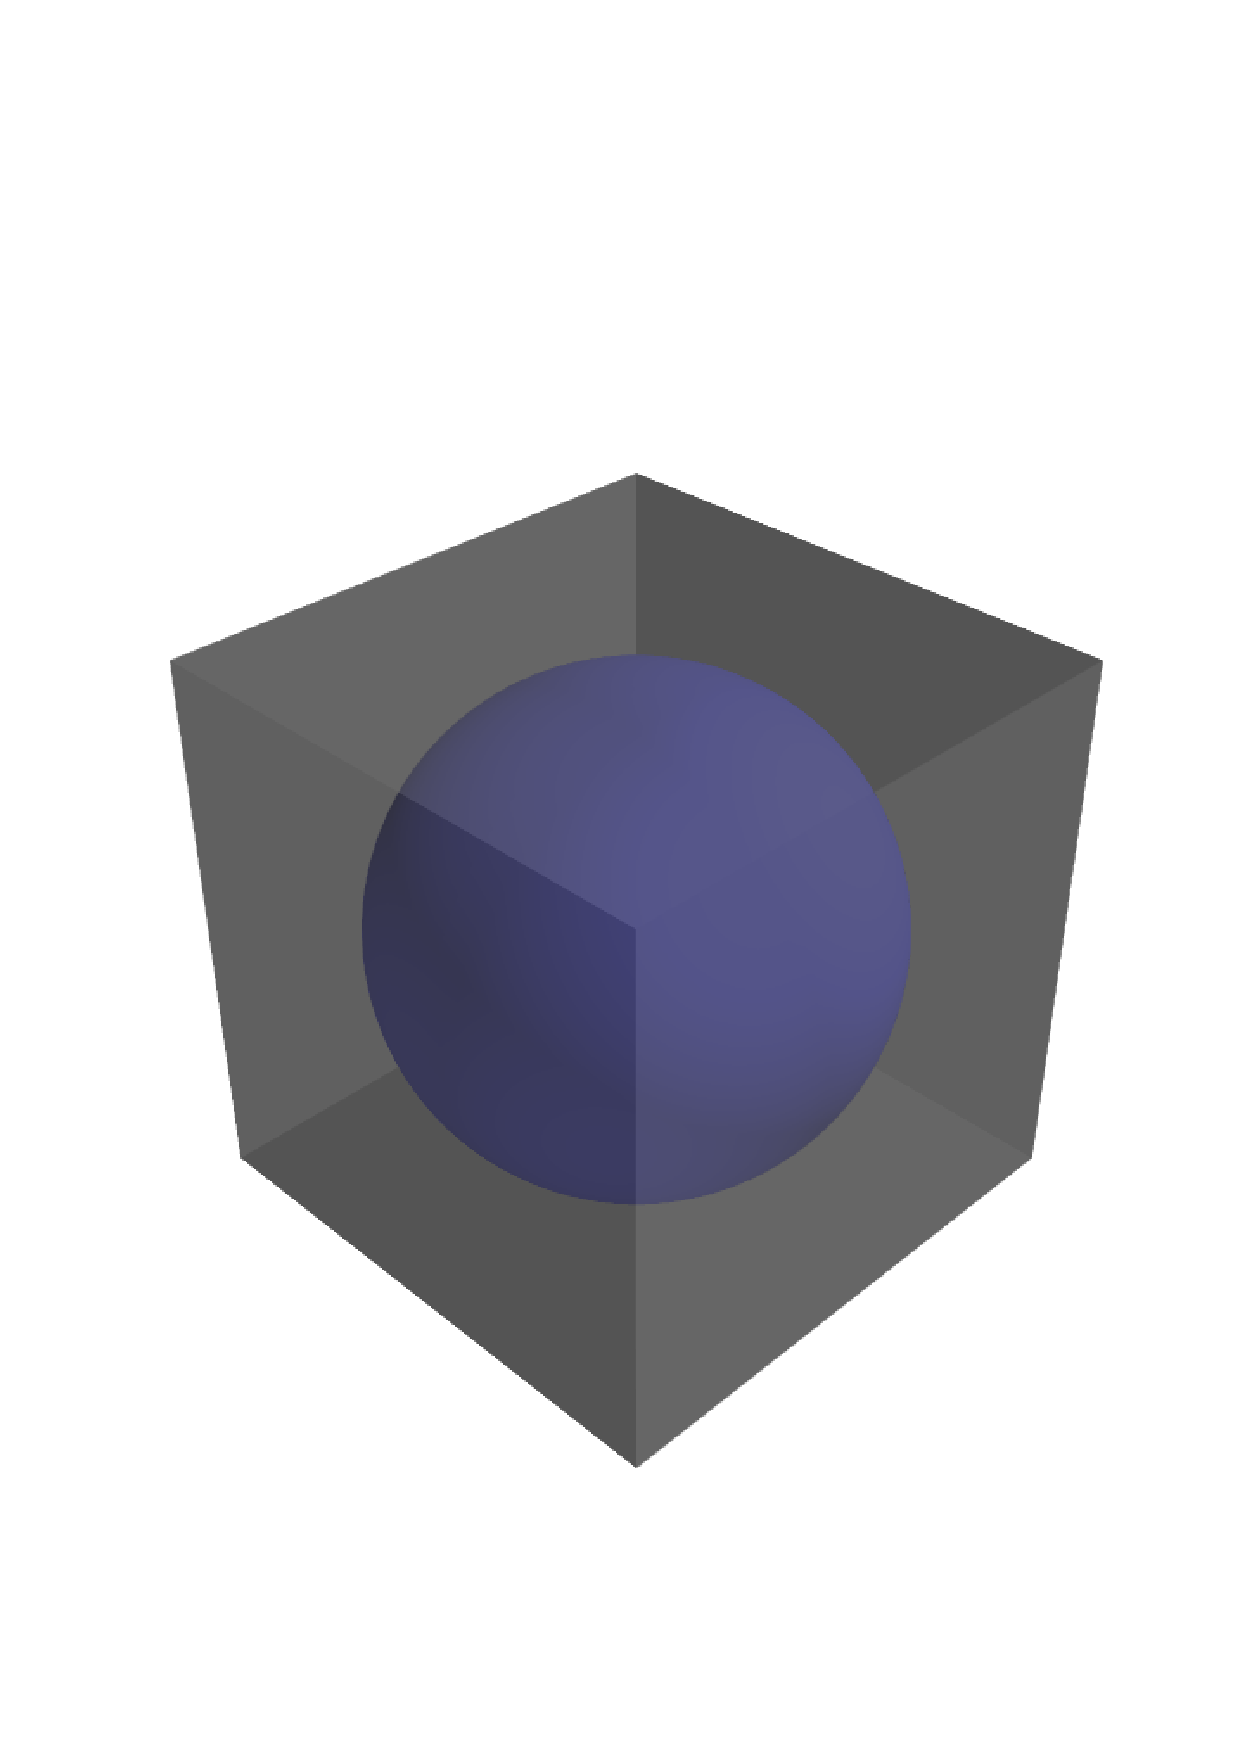
\includegraphics[width=\textwidth]{case1.pdf}
    \phantomcaption\label{subfig:sphere_A}
\end{subfigure}
\begin{subfigure}[b]{0.32\textwidth}
	  \begin{flushleft}
	  \large B
		\end{flushleft}
    \centering
    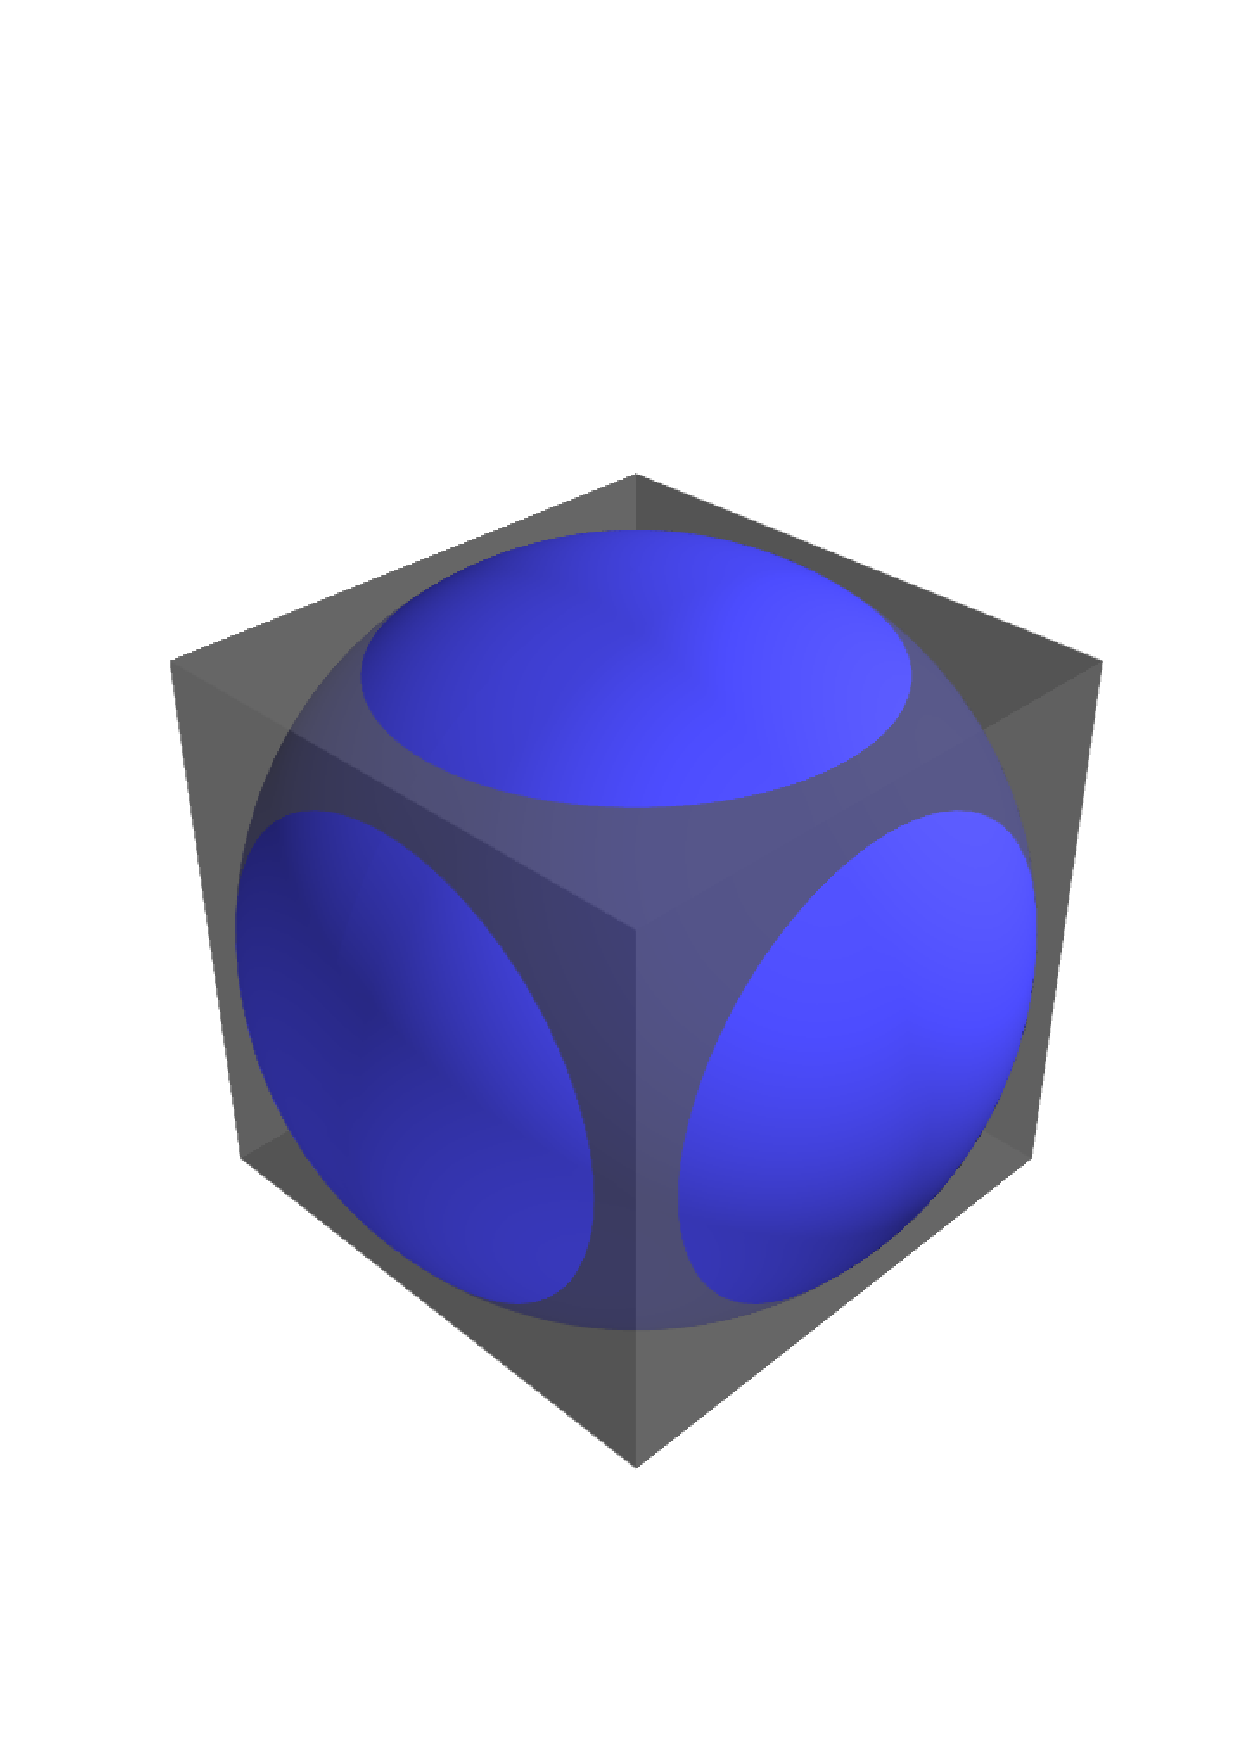
\includegraphics[width=\textwidth]{case2.pdf}
    \phantomcaption\label{subfig:sphere_B}
\end{subfigure}
\begin{subfigure}[b]{0.32\textwidth}
	  \begin{flushleft}
	  \large C
		\end{flushleft}
    \centering
    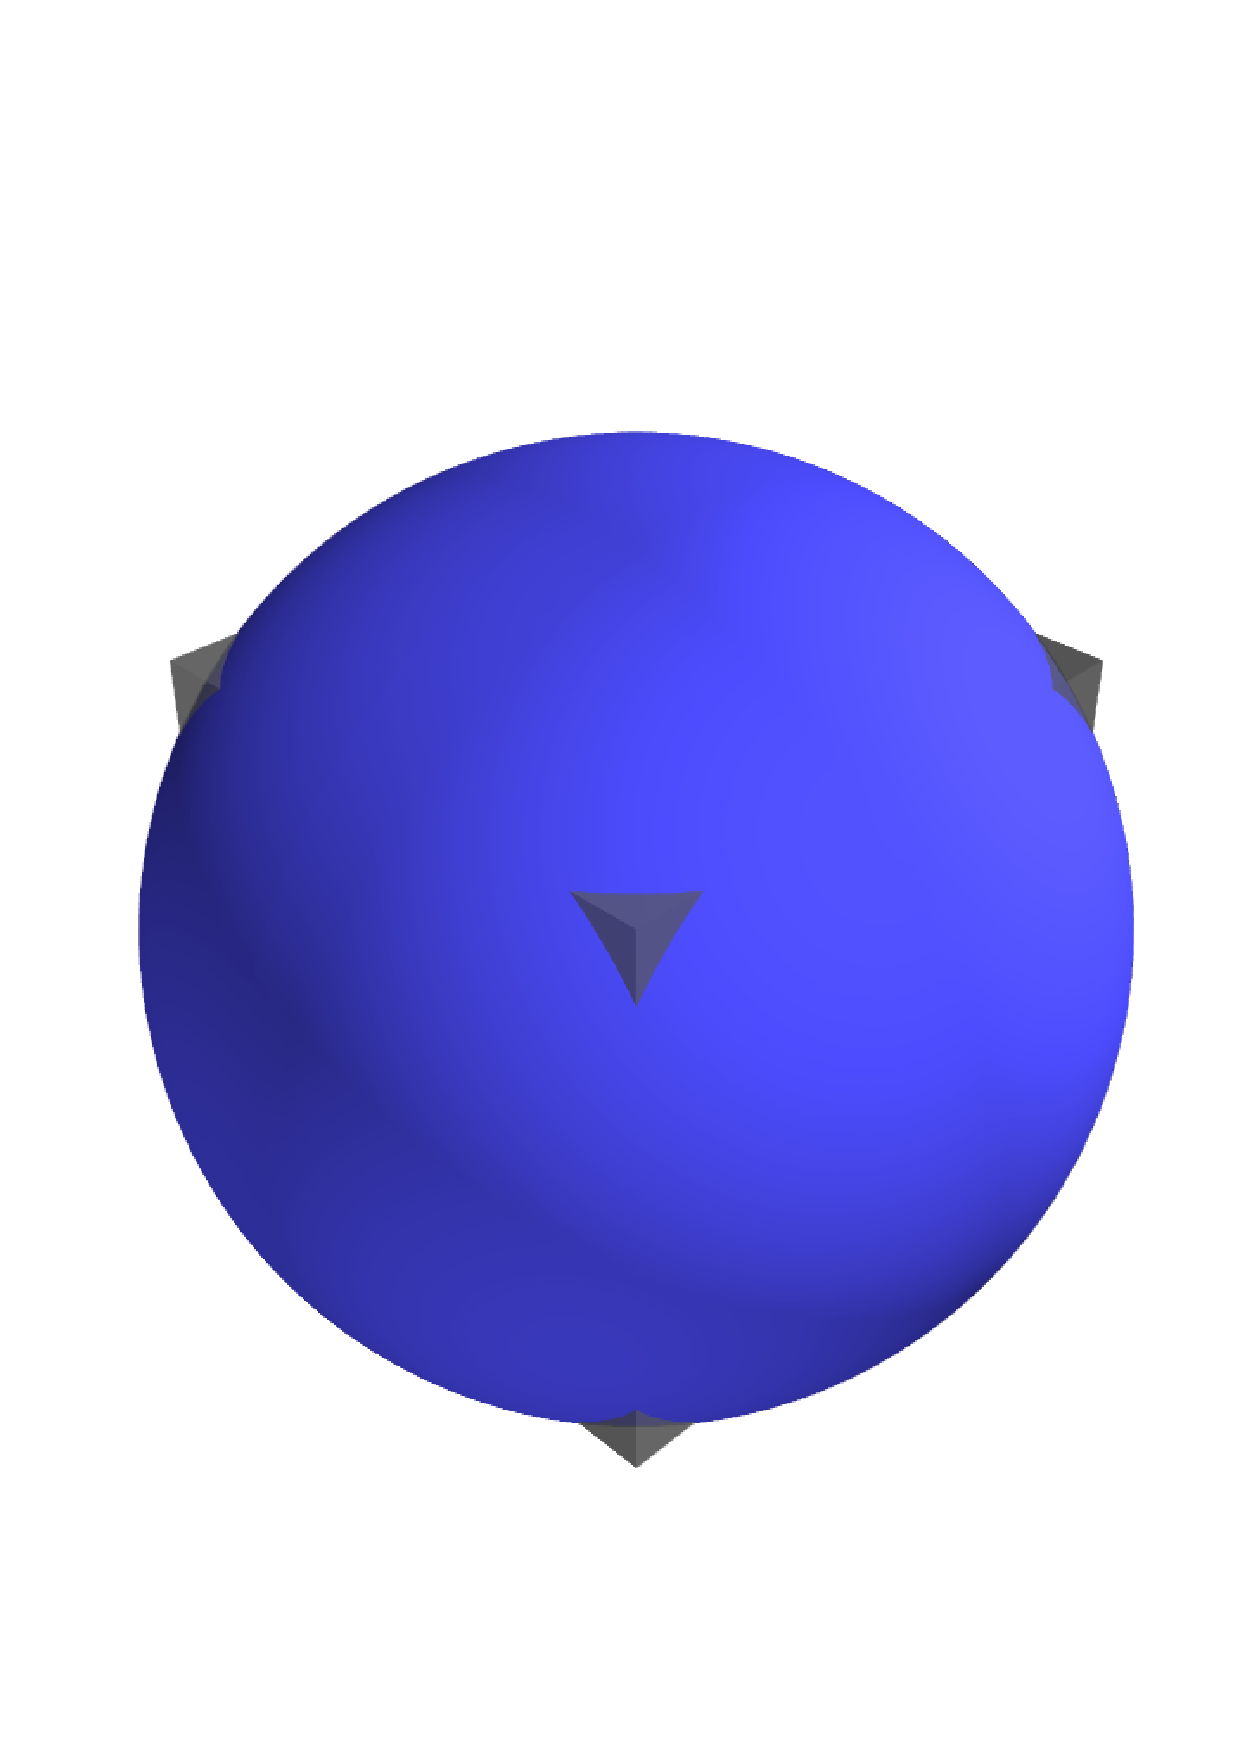
\includegraphics[width=\textwidth]{case3.pdf}
    \phantomcaption\label{subfig:sphere_C}
\end{subfigure}
\caption[Illustration of the effect of a cubic mask on the radial distribution function]{\subref{subfig:sphere_A}: For distances $D \in [0, L/2]$, the entire sphere is inside the cubic mask. \subref{subfig:sphere_B}: For $D \in (L/2, L/\sqrt{2}]$, only part of the sphere is inside the mask, while six spherical caps are outside. \subref{subfig:sphere_C}: For $D \in (L/\sqrt{2}, L\sqrt{3}/2]$, the six caps have ``grown'' to overlap each other.}
\label{fig:sphere}
\end{figure}
If we subtract the surface area $C$ of the spherical caps from the total area $A$, this overlap $E$ has been subtracted twice, and has to be added again. Calling the surface area of the sphere inside the cube $I$, we can write
\begin{equation}
I = A - 6C + 12E,
\end{equation}
where $A = 4\pi D^2$ and $C = 2\pi D\left(D-L/2\right)$. To find $E$, consider Figure \ref{fig:3D_mask_case3}.
\begin{figure}[h]
  \centering
  \includegraphics[width=0.6\textwidth]{3D_mask_case3.pdf}
  \caption[Illustration of the derivation of the surface area $E$ of the intersection between adjacent spherical caps]{Illustration of the derivation of the surface area $E$ of the intersection between adjacent spherical caps. The square is one of the cube's sides, and the circle outlines one of the spherical caps, a portion of the sphere bounded by the extended plane of the cube's side. The area $E$ is seen on the top of the figure, bisected by a great circle passing through points P and Q. The lines RP and RQ are also arcs of great circles. The surface area PQR is $2T$. The area $\frac{1}{2}E$ can be found by subtracting $2T$ from the fraction $\frac{2\gamma}{2\pi}$ of the surface area of the spherical cap bounded by RP and RQ.}
  \label{fig:3D_mask_case3}
\end{figure}
The circle outlines one of the spherical caps, sitting on top of one of the cube's sides. The sphere intersects one of the cube's edges at points P and Q. A great circle passing through P and Q bisects the area $E$ into two equal halves. Two more great circles pass through the center point R on the cap's surface and P and Q, respectively. The spherical triangle PQR is further bisected into two equal spherical triangles by a fourth great circle passing through R. One such half (blue triangle in the figure) has a surface area $T = D^2\left( \alpha+\beta+\gamma-\pi \right)$, where $\alpha$, $\beta$, and $\gamma$ are the corner angles. The area $\frac{1}{2}E$ can now be found by subtracting $2T$ from the fraction $2\gamma/2\pi$ of the spherical cap's surface area $C$ which is bounded by the two great circle arcs RP and RQ, i.e., $E = 2\left( (2\gamma/2\pi)C - 2T \right)$. The area $I$ of the sphere inside the cube is therefore
\begin{eqnarray}
I &=& A - 6C + 12E \\
  &=& A - 6C + 12\left( 2\left( \tfrac{2\gamma}{2\pi}C - 2T \right) \right) \\
  &=& A - 6C\left( 1 - \tfrac{\gamma}{\pi} \right) - 48T.
\end{eqnarray}
Summarizing, the RDF is
\begin{equation}
\rho(D) = 
\begin{cases}
   \rho_0 A   &   \text{for } 0 \le D \le \frac{L}{2} \\ 
   \rho_0 \left(A - 6C\right)   &   \text{for } \frac{L}{2} < D \le \frac{L}{\sqrt{2}} \\
   \rho_0 \left(A - 6C\left( 1 - \tfrac{\gamma}{\pi} \right) - 48T \right)   &   \text{for } \frac{L}{\sqrt{2}} < D \le \frac{L\sqrt{3}}{2} \\
   0 & \text{otherwise},
\end{cases}
\end{equation}
where
\begin{eqnarray}
A &=& 4\pi D^2 \\
C &=& 2\pi D \left(D-\tfrac{L}{2}\right) \\
T &=& D^2\left( \alpha+\beta+\gamma-\pi \right) \\
\alpha &=& \text{sin}^{-1}\left( 1 / \sqrt{2 - \tfrac{L^2}{2D^2}} \right) \\
\beta  &=& \tfrac{\pi}{2} \\
\gamma &=& \text{sin}^{-1}\left(  \sqrt{(1 - \tfrac{L^2}{2D^2}) / (1 - \tfrac{L^2}{4D^2})}  \right) .
\end{eqnarray}
As before, the PDF $f(D)$ of source-target distances is the normalized product of the RDF $\rho(D)$ and some kernel $\mathcal{P}(D)$, and the CDF $F(D)$ can be found by numerical integration of $f(D)$. Figure \ref{fig:3Dex} shows an exemplary PDF and CDF, together with the corresponding connectivity pattern. 

\begin{figure}[ht]
\centering
\begin{subfigure}[b]{0.49\textwidth}
	  \begin{flushleft}
	  \large A
		\end{flushleft}
    \centering
    \includegraphics[width=\textwidth]{Gaussian3D_PDF.pdf}
    \phantomcaption\label{subfig:gaussian3D_PDF}
\end{subfigure}
\begin{subfigure}[b]{0.49\textwidth}
	  \begin{flushleft}
	  \large B
		\end{flushleft}
    \centering
    \includegraphics[width=\textwidth]{Gaussian3D_CDF.pdf}
    \phantomcaption\label{subfig:gaussian3D_CDF}
\end{subfigure}
\begin{subfigure}[b]{0.60\textwidth}
	  \begin{flushleft}
	  \large C
		\end{flushleft}
    \centering
    \includegraphics[width=\textwidth]{Gaussian3D_network.png}
    \phantomcaption\label{subfig:gaussian3D_network}
\end{subfigure}
\caption[Exemplary PDF, CDF and connectivity pattern for a network in 3D space, using a Gaussian kernel]{Exemplary PDF (\subref{subfig:gaussian3D_PDF}), CDF (\subref{subfig:gaussian3D_CDF}) and connectivity pattern (\subref{subfig:gaussian3D_network}) for a spatially structured network in 3D space. A Gaussian kernel is used, and the layer and mask size is $L^3 = 1$.}
\label{fig:3Dex}
\end{figure}

The KS test is used to compare this theoretical CDF with the observed EDF. A $Z$-test that compares the observed number of connections with the expected number is also implemented. It works the same way as the $Z$-test implemented for 2D layers.



\subsection{Implementation\label{subsec:3Dimp}}

A script implementing the test procedure can be found in Appendix \ref{app:3D}. The usage is similar to that of 2D layers, and is demonstrated in the main section of the module. Unless \inline{kernel_params} is specified, suitable defaults are used.  



\subsection{Results\label{subsec:3D_res}}

\graphicspath{{figs/spatial/3D_results/}}

Using the script in Appendix \ref{app:3D}, NEST's connection algorithm for 3D spatially structured networks can be tested. With $L = 1$, $N =$ 1,000,000, there appears to be close agreement between the expected and the observed distribution of source-target distances for all four kernels (constant: $p = 0.726$, linear: $p = 0.978$, exponential: $p = 0.803$, and Gaussian: $p = 0.770$). The theoretical and observed PDF and CDF for constant kernel are shown in Figure \ref{fig:res_constant3D}. 
\begin{figure}[t]
\centering
\begin{subfigure}[b]{0.49\textwidth}
	  \begin{flushleft}
	  \large A
		\end{flushleft}
    \centering
    \includegraphics[width=\textwidth]{3D_constant_PDF.pdf}
    \phantomcaption\label{subfig:res_3D_constant_PDF}
\end{subfigure}
\begin{subfigure}[b]{0.49\textwidth}
	  \begin{flushleft}
	  \large B
		\end{flushleft}
    \centering
    \includegraphics[width=\textwidth]{3D_constant_CDF.pdf}
    \phantomcaption\label{subfig:res_3D_constant_CDF}
\end{subfigure}
\caption[Theoretical and empirical PDF and CDF of source-target distances using a constant kernel]{PDF (\subref{subfig:res_3D_constant_PDF}) and CDF (\subref{subfig:res_3D_constant_CDF}) of source-target distances, with layer size $L^3=1$, using the constant kernel. The grey lines show the theoretical predictions, and the red lines show the empirical observations. The empirical PDF is plotted with 100 bins.}
\label{fig:res_constant3D}
\end{figure}
When the source node is moved to ($L$/4, $L$/4, $L$/4) so that the periodic boundary conditions come into play, there is still a close agreement between theory and observation (constant: $p = 0.965$, linear: $p = 0.367$, exponential: $p = 0.217$, and Gaussian: $p = 0.707$), and the same holds when the number of VPs is increased to 4 (constant: $p = 0.726$, linear: $p = 0.600$, exponential: $p = 0.852$, and Gaussian: $p = 0.561$).



\subsubsection{Sensitivity}

The same control algorithm that was implemented for 2D layers is implemented for 3D layers. It can be used both with the KS test and with the $Z$-test. We use it again to test the sensitivity of the test procedure to the same biases as for 2D layers. As before, we note that the reported $p$-values are only examples. 

The first bias, introduced by having the Gaussian kernel function return a too high value, with a constant $c = 0.01$ added, was detected by the KS test with $N =$ 1,000,000 ($p = 1.52\times 10^{-56}$) and $N =$ 100,000 ($p = 1.48\times 10^{-6}$), but not with $N =$ 10,000 ($p = 0.350$). It was detected by the $Z$-test with $N =$ 10,000 ($p = 6.25\times 10^{-5}$) as well as with larger $N$, but not with $N =$ 1,000.

The second bias, where the distances passed to the Gaussian kernel function are too high by 1\%, is detected by the KS test with $N =$ 1,000,000 ($p = 1.40\times 10^{-9}$) and $N =$ 100,000 (at significance level $\alpha = 0.05$; $p = 0.019$), but not with $N =$ 10,000. The $Z$-test also detects the bias with $N =$ 100,000 ($p = 5.46\times 10^{-8}$), but not with $N =$ 10,000 ($p = 0.818$).

The third bias, where a randomly selected 1\% of the nodes are excluded as potential targets, can not be detected by the KS test, regardless of $N$. The $Z$-test, however, detects the bias with $N =$ 1,000,000 ($p = 3.38\times 10^{-10}$), $N =$ 100,000 ($p = 1.05 \times 10^{-4}$), and $N =$ 10,000 (at $\alpha = 0.05$; $p = 0.035$), but not with $N =$ 1,000 ($p = 0.388$).

Overall, the KS test is sensitive when $N$ is large, but the sensitivity falls of rapidly with decreasing $N$. Perhaps surprisingly, the $Z$-test is often more sensitive than the KS test, depending on the nature of the bias we wish to detect. The two tests are in some ways complementary to each other. The KS test detects biases that changes the overall distribution of source-target distances, but it does not detect biases that affect the total number of connections without changing the distribution. The $Z$-test does detects biases that affect the total number of connections without changing the distribution. 

\graphicspath{{figs/spatial}}



\section{Automated test procedure\label{sec:auto_spatial}}

We will now describe the automated test procedure for spatially structured networks, both in 2D and 3D space.

To maintain a high sensitivity while reducing the rate of false positives and the execution time, an adaptive testing strategy is used. First, a single KS test is run. If the resulting $p$-value is suspiciously low, a two-level test is run, comparing the output of $n_\text{runs}$ KS tests to the expected uniform distribution, thereby either confirming or allaying our suspicion. 

As discussed earlier, certain errors can not be detected by the KS test, but are detected by the $Z$-test. We therefore include the $Z$-test in the automated test procedure. The adaptive strategy can be used for the $Z$-test as well as for the KS test, re-running the $Z$-test $n_\text{runs}$ times if the first test results in a suspicious $p$-value.

Let $\alpha_1$ be the value below which the $p$-value from the single KS test (or $Z$-test) is considered suspicious, and $\alpha_2$ be the value below which the $p$-value from the two-level test is considered too extreme, resulting in the rejection of $H_0$. The fraction of false positives will be $\alpha = \alpha_1 \alpha_2$. If $k$ tests are included in the test suite, the number of false positives is binomially distributed. The probability of seeing one or more false positives is therefore 
\begin{eqnarray*}
\Prob{x \ge 1} &=& 1 - \Prob{x=0} \\
               &=& 1 - \binom{k}{0} (\alpha_1 \alpha_2)^{0} (1-\alpha_1 \alpha_2)^{k} \\
               &=& 1 - (1 - \alpha_1 \alpha_2)^{k}
\end{eqnarray*}
The choice of $\alpha_1$ and $\alpha_2$ might thus depend on $k$, as well as other factors, such as the acceptable rate of false positives and the desired sensitivity and the tests. The number of nodes $N$ in the network and number of re-runs $n_\text{runs}$ upon suspicion must also be chosen. Large values will clearly increase sensitivity, but the available computation time is a limiting factor.  



\subsection{Implementation\label{subsec:autoimp_spatial}}

An implementation of the automated test procedure is found in Appendix \ref{app:unit-spatial}. Each of the four kernels (constant, linear, exponential, and Gaussian) are tested. In addition, tests are done with the source node shifted away from the center, and with multiple VPs. These six test configurations are tested both with the KS test and the $Z$-test, and both in two-dimensional and three-dimensional space. A total of 24 tests is thus run. With $\alpha_1 = \alpha_2 = 0.01$, the entire test suite will falsely report a problem with a probability $1 - (1 - 0.01\times 0.01)^{24} = 2.40 \times 10^{-3}$. With $N =$ 100,000 nodes in the network and $n_\text{runs} = 100$ re-runs upon suspicion, the test suite will in most cases complete in a couple of minutes.



\clearchapter

